\documentclass{article}

\usepackage[utf8]{inputenc}
\usepackage{graphicx}
\usepackage{caption}
\usepackage{subcaption}

\begin{document}

\section*{Introduction}
For this practical session, we use Kmeans to cluster data based on their locations to find all attractive regions.
%
We used python to process our data, train our model and predict.
%
Our data set came from Flick which is a Yahoo photo sharing system and consists of locations, upload time, user id and description, etc.. 
%
But we just used the locations we wanted to find attractive regions.
%
We found that we have to set the size of different clusterings to find the clearest results.

\par

At first we got our results and just plotted it without map. We just wanted to make sure it worked.
%
The first time we converted many columns to one column, "date upload time" and used a category to represent it.
%
And we trained based on location, user id, picture id and upload time.  
%
The point cloud we got was really fuzzy, there was no cluster to see.
%
Finally, we found that this was caused by too many non relevant columns used in the training data.
%
After we dropped some other columns except locations, it was very clear.
%
We could get something explicitly through out plotting.

\par
After we finished this, we added our map as background.
%
And we grouped them based on the same predict result and ploted group by group.
%
We found that tete d'or park and bellecour were really attractive.
 
\section*{Implementation}
\par
To achieve our results, we decided to just implement clustering in Python without KNIME. Immediately we ran into issues with the size of the the initial dataset.
When looking at the .csv file in the PyCharm IDE, the whole IDE would freeze. After realizing that this was our problem and not Pythons processing 
ability, we moved on. Our first step was to build date taken and date upload from the current columns in the dataset. Since it was not well 
represented initial, this was to be done first. After our new columns replaced the old ones we still had too many columns. As pointed out 
by someone in our class, there were a lot of repeated columns. This was easy to add in and made our dataset go from 167702 
data points to just 13504. 
\par 
Now we can implement clustering. We started out using the K-Means clustering algorithm. Once we ran the code, we waited and waited and waited.
Clearing there was too many iterations and too much data to be processed. We tried minimizing the data as much as possible however, nothing
was fixing the computation time. Luckily, there was MiniBatchKMeans which splits the dataset into small batches for faster computation. 
Based on the sckit API there was little to no different between the two implementations. After we were able to let the 
clustering algorithm run efficiently, we then plotted our data. We started off our clustering by using the latitude, longitute, and upload date and time. 
However, this gave us some weird results on our graph. The clusters were very undefined and it seemed like it wasn't working. Then it was
clear that including the upload and taken dates were causing the undefined clusters. We removed them from the computation of the clustering, and 
we just used latitude and longitute. This resulted in much clearer results. We could see clear separations of our data. But at this point, 
we were plotting the values to a blank plot. But these were coordinates on a map, so we took a picture of a map that was defined by our coordinates
and used it as the background to our scatter plot. This was not the best solution but it was good enough for us to interpret the data as a location. 
Once we had completed our program, we then created multiple graphs using different sized clusters for analysis. 


\section*{Results}
Once we had all the components working together in our Python project we then made a few maps to analyze. We made 5 maps of increasing clustering size for comparison. Starting with 8 clustering and going all the way up to 50 gave us a good range of how many clusters were needed to have good results. 

\par
Starting with 8 clusters we can see some good separation in the data, see Figure \ref{fig:clusters_8}. If we look on the outer edges of the map all of the clusters are very well defined and have no jarring cuts and is enough to distinguish good groups. But also since these clusters are so separated they good be split up even more with more clusters. As for the main two clusters in the middle there is a weird split in the middle which is clearing trying to separate north and south. Since it is just a harsh cut and there is no good reason for it we knew this was not the best clustering possible. 

\par 
The 16 clustering achieved similar results with the 8 clusters, see Figure \ref{fig:clusters_16}. It preforms a little bit better by making a better split in the middle of the map. Half of it is downtown Lyon and the other half is more towards park tete d'or. Theses are obvious areas where events happen all the time and would cause many photos to be taken. In regards to the outer areas of the map, 16 clusters even better defines these different groups of images taken and has very little over lap. 

\par 
For the next two clustering we used 26 and 32. They preformed similarly in the outer areas. This is to be expected since the groups are more clear and farther apart and easier to be predicted. Whats most different between the 26 and 32 clusters this the center of Lyon area. The 26 cluster makes a clear difference between the island and the right half of Lyon right where the river is located. This is great and expected. Whats odd is the splitting of the brown data points from the top of the map with the rest of the brown data points on the left. As seen in Figure \ref{fig:clusters_26_zoomed}, this is odd because it seems as though it should be two or three different clusters. This is where the 32 clusters preformed better as seen in Figure \ref{fig:clusters_32_zoomed}. It makes a red cluster right on top of park tete d'or. This is exactly what we were looking for! There is a clear grouping of the different areas of Lyon where big events would happen and cause many pictures to be taken. 

\par 
Finally, in Figure \ref{fig:clusters_50}, we can see many clusters in the middle of the map. These are not as well defined as some of the lower count clusters. This was most likely do to the actual input data. We know that more clusters is better but since there is no additional information or better prediction method its hard to clear clusters to be made in such dense areas. So for now we assume that to make the best prediction of clusters we would use less clusters than 50 and add more information to Kmeans for the best results. 

\section*{Conclusion}
In conclusion, we were able to create good clusters that were defined by clear geographical locations where events would take place in Lyon. We attempted to use many different cluster sizes for analysis and comparison. From this we learned that for the best predictions more clusters are better but too many might be pushing the ability of the predictor. Something that we noticed as we were making the predictions of different clustering sizes, is that each prediction was slightly different for the same cluster size. This was kind of surprising because the differences weren't small. For example, when clustering with 16 clusters, we ran it many many times, because the outer edges of the map were garnering odd groups that over lapped or over generalized. Which means that the data was too varying and far apart and required interpretation. In fact, many of our maps required some human interpretation of the clusters. In the end we can't just assume that the clusters it makes will be perfect or well defined. The clustering helps guide us to the right areas of geographical significance, but human interpretation is absolutely nessecary. 


%\ref{fig:clusters_8}
\begin{figure}[!h]
  \centering
  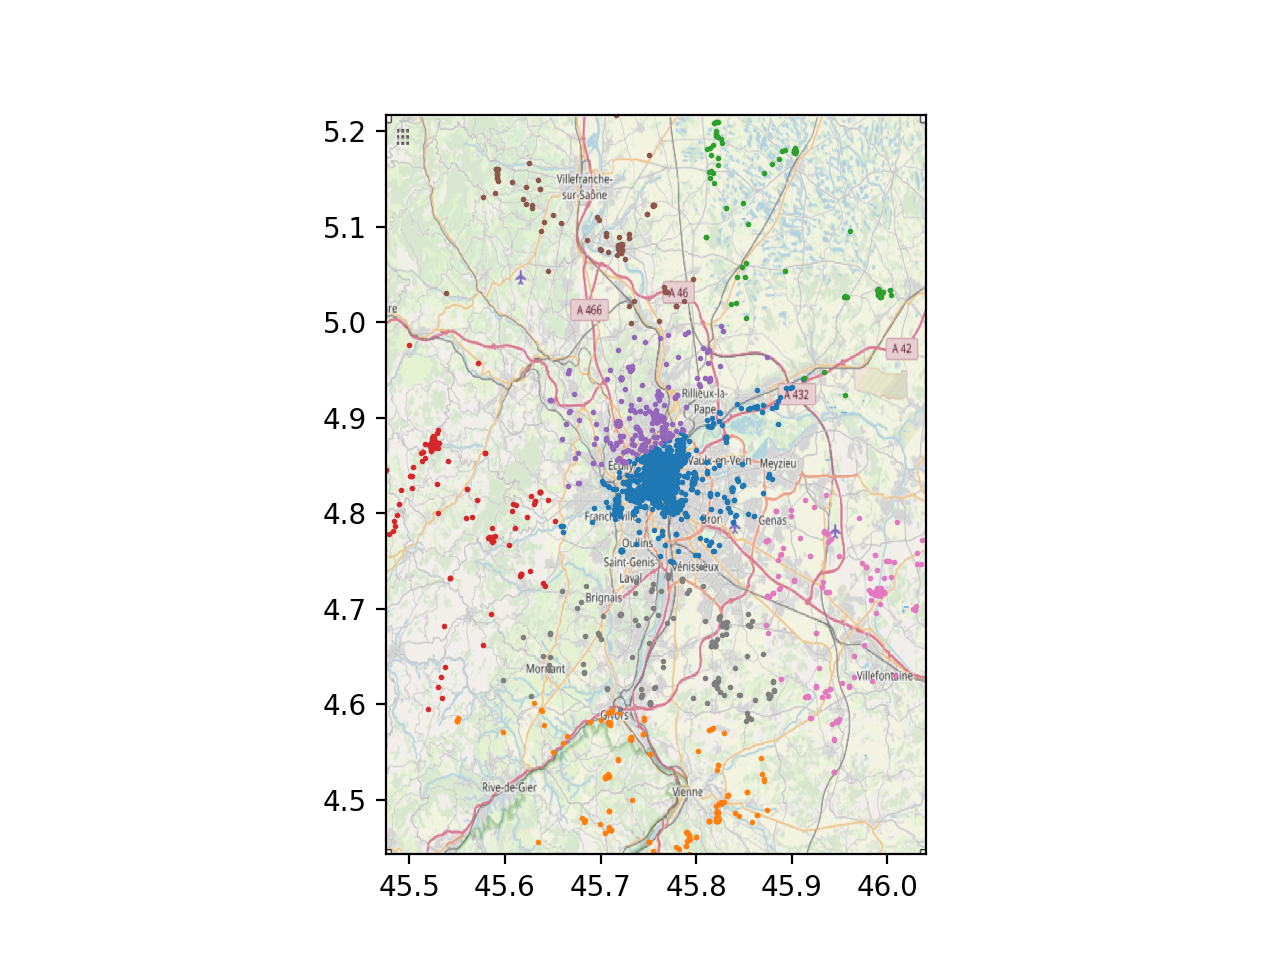
\includegraphics[width=0.5\textwidth]{small_clusters_8.png}
  \caption{clusters size is 8}
  \label{fig:clusters_8}
\end{figure}


\begin{figure}[!h]
  \centering
  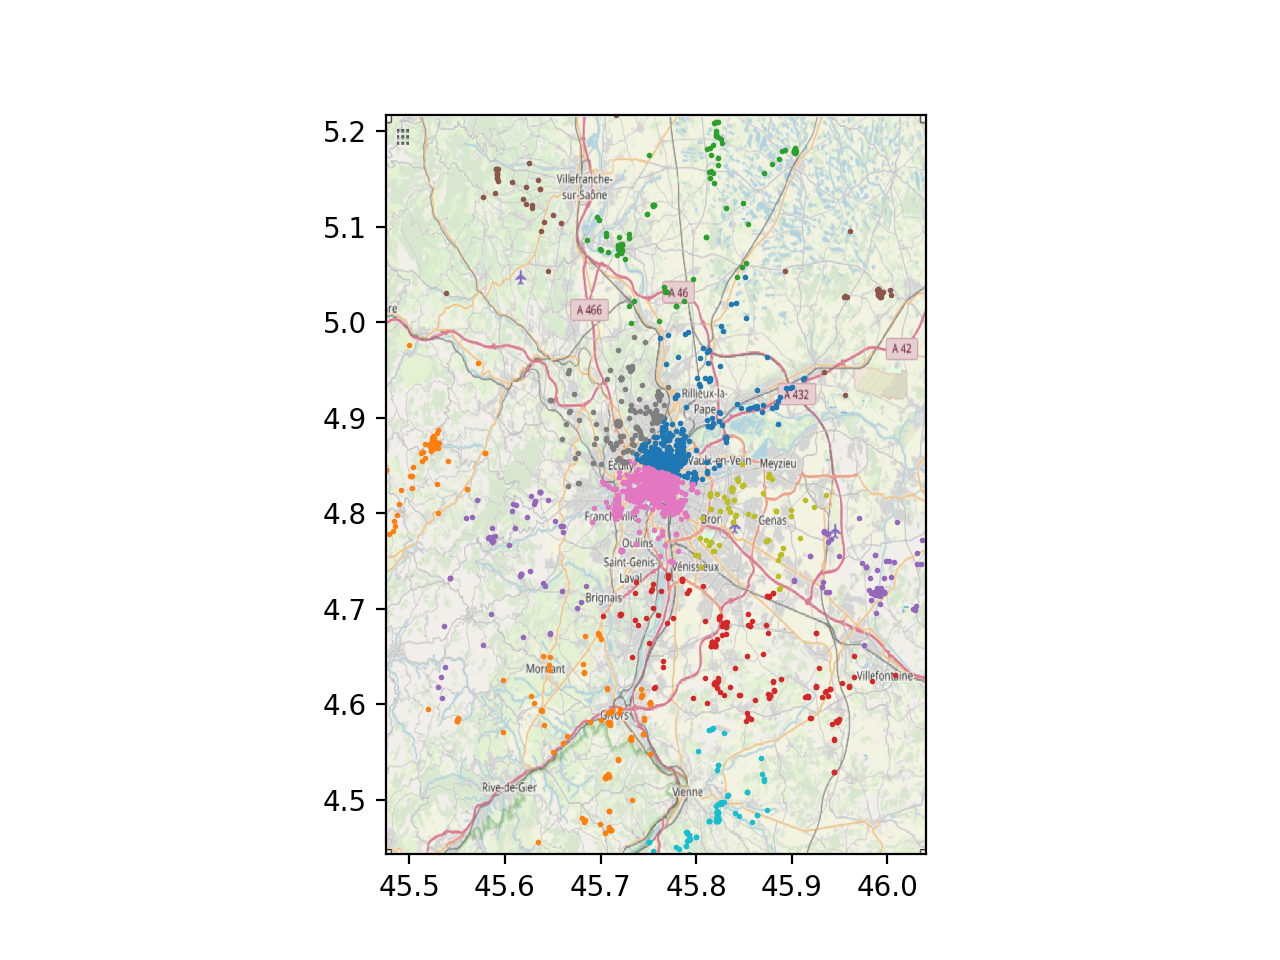
\includegraphics[width=0.5\textwidth]{medium_clusters_16.png}
  \caption{clusters size is 16}
	\label{fig:clusters_16}
\end{figure}

\begin{figure}[!h]
  \centering
  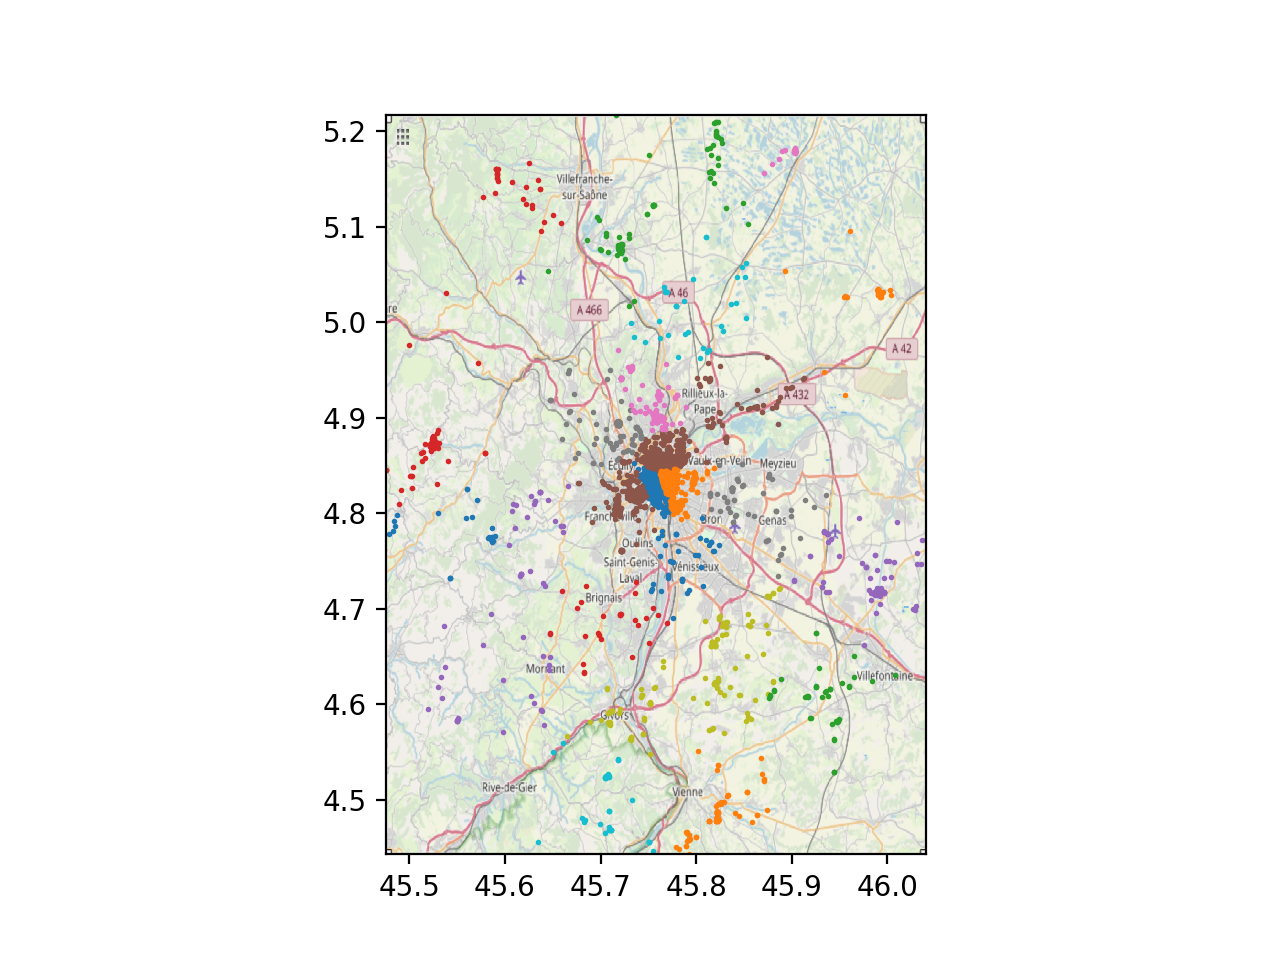
\includegraphics[width=0.5\textwidth]{clustering_26_full.png}
  \caption{clusters size is 26 full}
	\label{fig:clusters_26_full}
\end{figure}

\begin{figure}[!h]
  \centering
  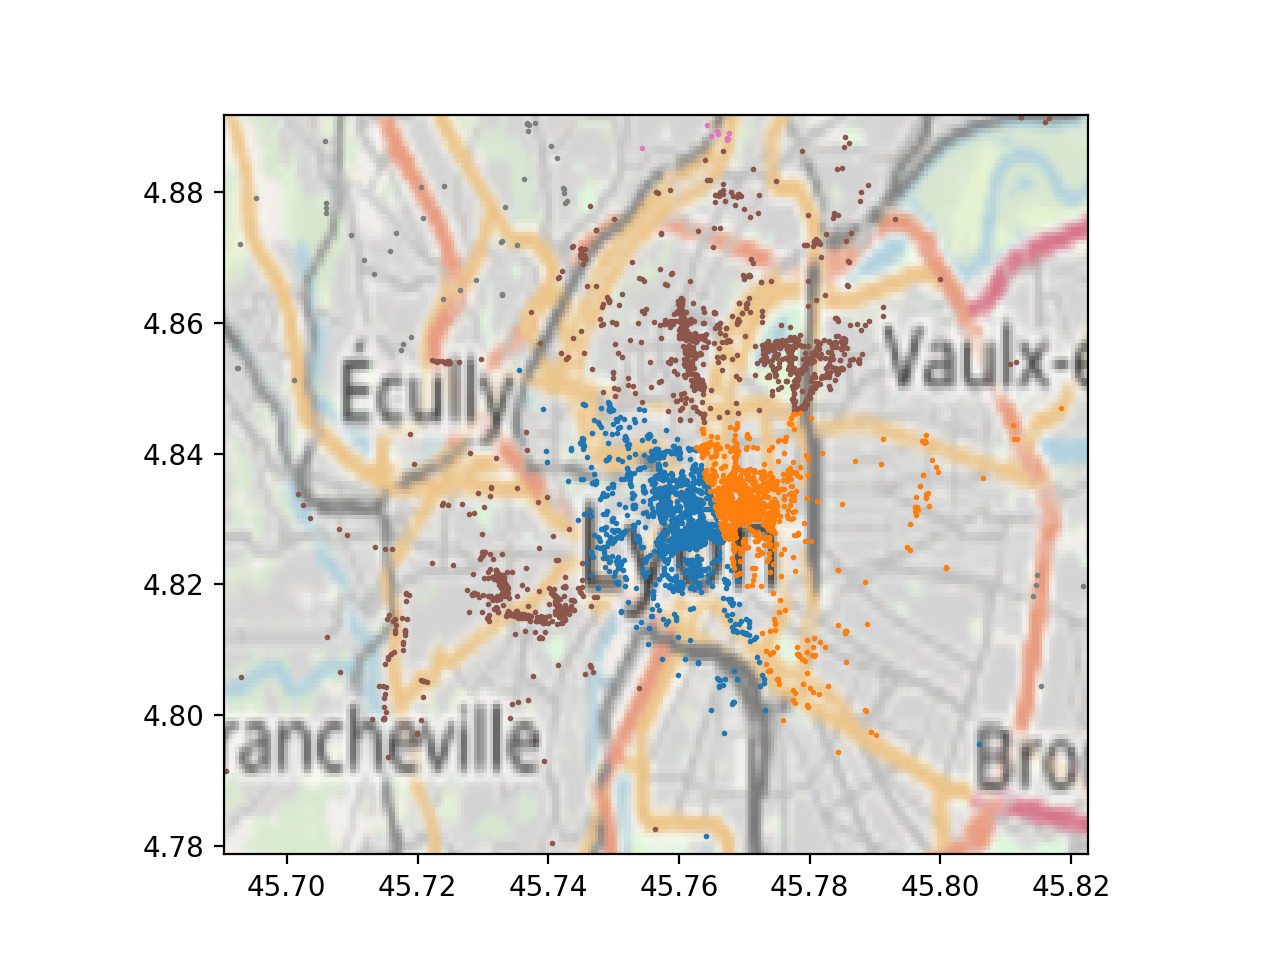
\includegraphics[width=0.5\textwidth]{clustering_26_zoomed.png}
  \caption{clusters size is 26 and zoomed}
	\label{fig:clusters_26_zoomed}
\end{figure}

\begin{figure}[!h]
  \centering
  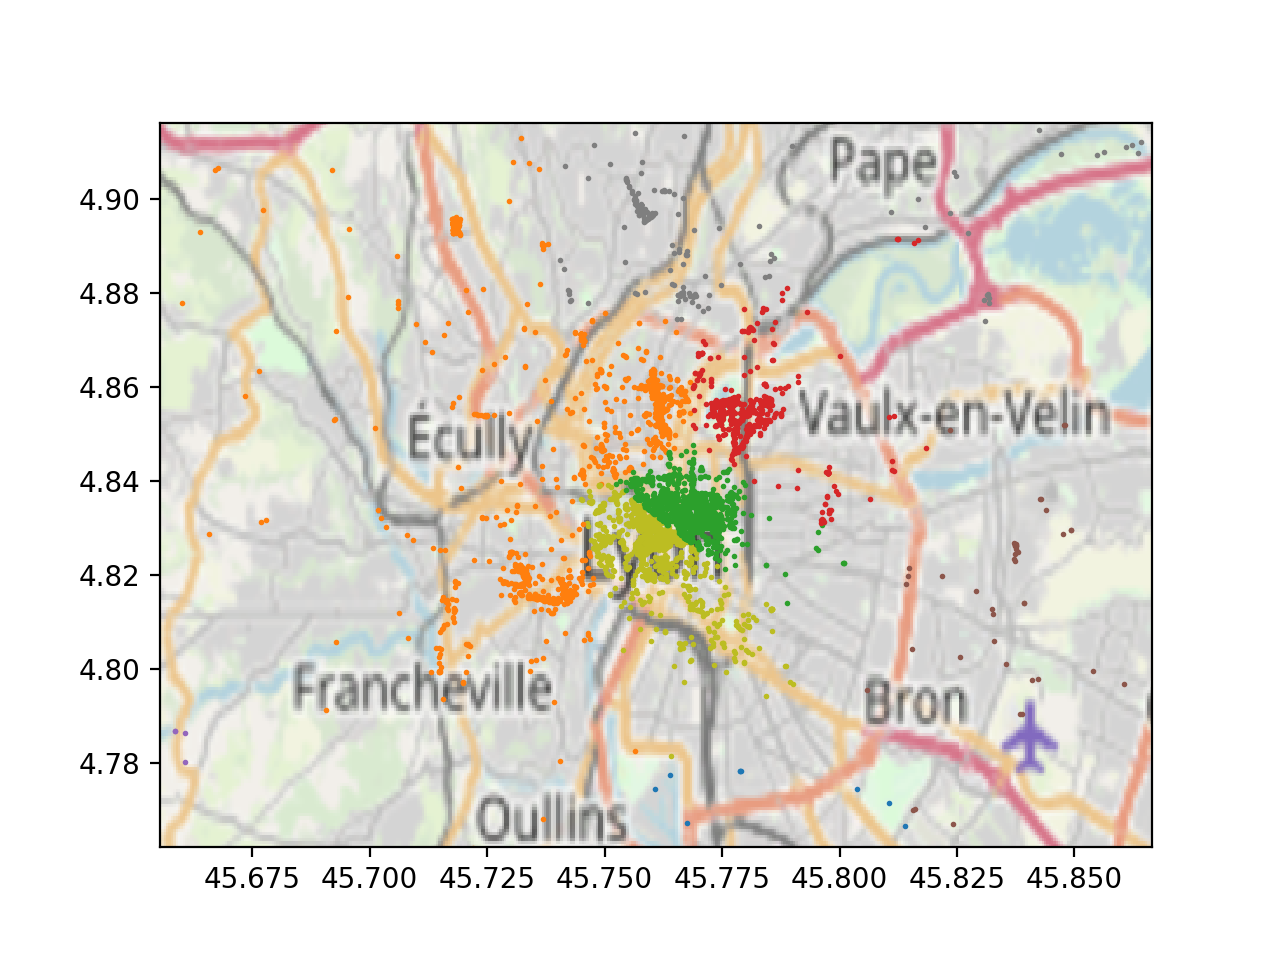
\includegraphics[width=0.5\textwidth]{clustering_32_zoomed.png}
  \caption{clusters size is 32 and zoomed}
	\label{fig:clusters_32_zoomed}
\end{figure}

\begin{figure}[!h]
  \centering
  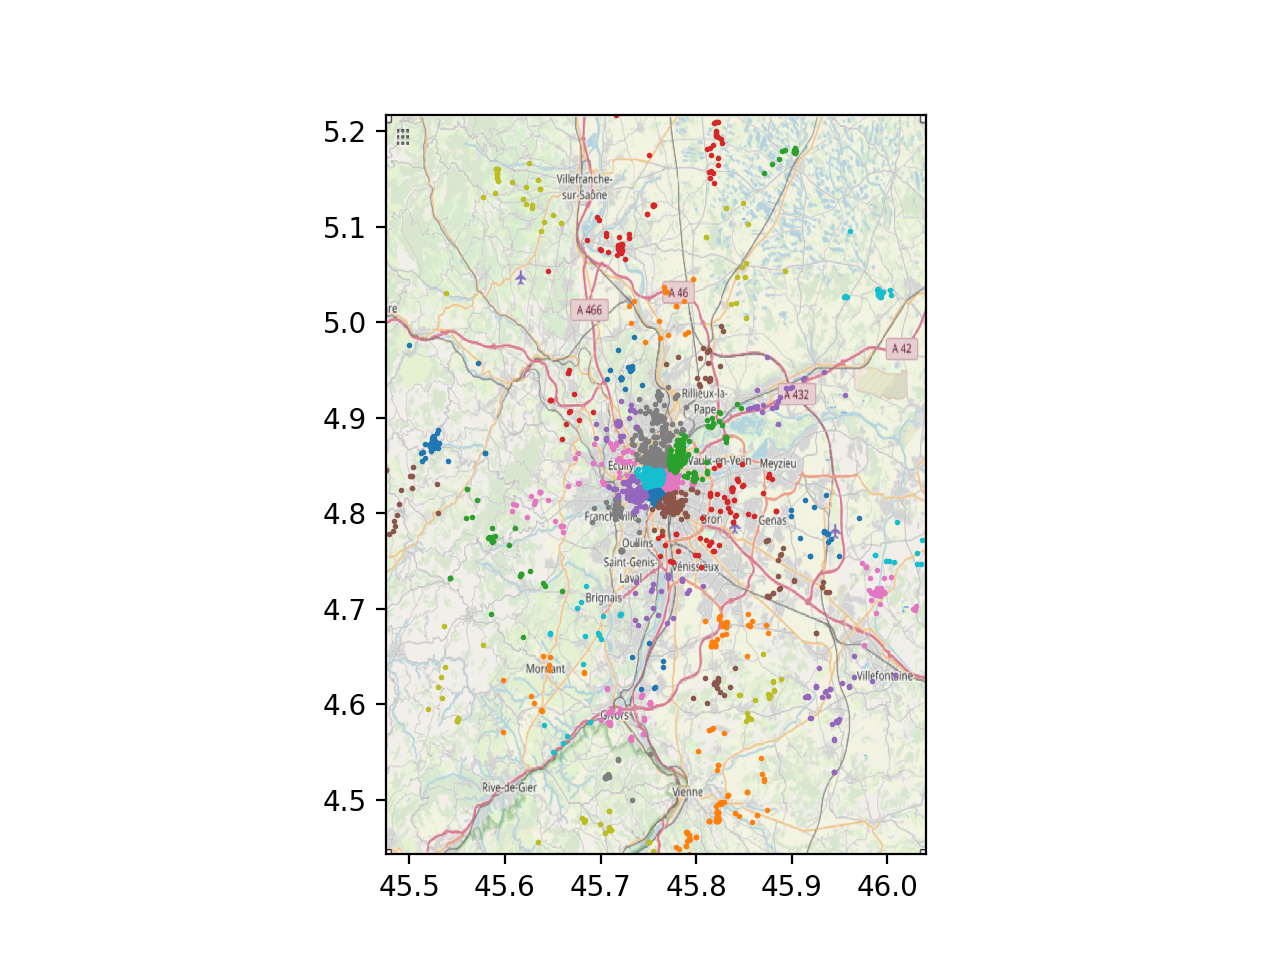
\includegraphics[width=0.5\textwidth]{clustering_50.png}
  \caption{clusters size is 50}
	\label{fig:clusters_50}
\end{figure}








\end{document}
